% Numerical provenance: research/output-review-2026-11-06/results.json and
% kaggle-roadmap-2026-10-31/{local-plan.json,EXECUTION-PROTOCOL.md,degron_v3/}.
\subsection{Research Campaign and Recovery Design}\label{sec:campaign-methods}
The execution unit is a dependency-tracked job with pinned code, data, model revision, protocol and
runtime identity. The Kaggle run supplies the reference experiments; the Windows successor expands
the pLM family and completes a matched frozen--LoRA comparison. These runs use the same development
population, but different software and GPU environments. They are retained as separate estimates.

Figure~\ref{fig:campaign-lineage} shows how interrupted work is recovered. Completed outputs can be
inherited only after compatibility and checksum checks. The tokenizer-repair successor reuses 456
completed jobs from the earlier local campaign; it does not count those jobs twice. Paused training
uses committed checkpoints, including optimiser and random-state information. A timer-failure run
that produced no scientific OOF predictions is superseded. A final report job denotes completion of
the runnable graph; missing reviewed external and structure inputs remain explicit pending states.

\begin{figure}[htbp]
  \centering
  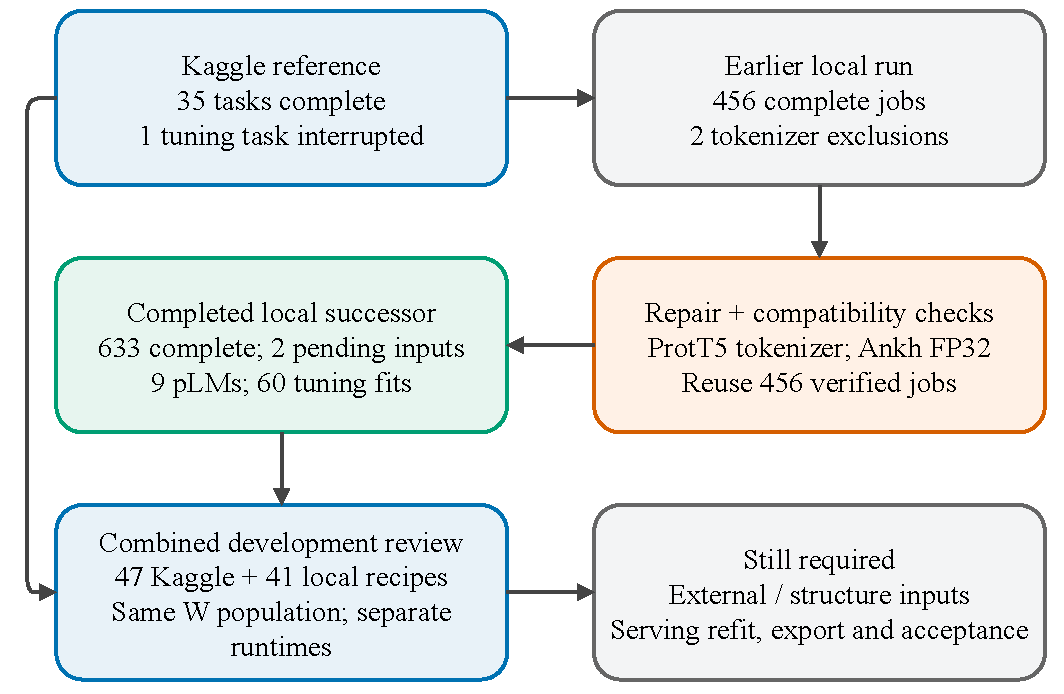
\includegraphics[width=\textwidth]{assets/diagrams/campaign-2026-11-06/campaign-lineage.pdf}
  \caption{Campaign lineage and evidence roles at completion on 6 November 2026.
  Inheritance preserves compatible work; the combined review does not create independent datasets.}
  \label{fig:campaign-lineage}
\end{figure}

\subsection{Nested Selection and Prediction Aggregation}
The evaluation unit is a mutation cell, while splitting and uncertainty respect protein groups.
The full-PSI development set W contains 235 peptides, 221 groups and 122,412 cells. Five fixed outer
folds are shared across recipes. Seeds 17, 29 and 43 vary the inner group split and stochastic fitting;
they do not provide three independent outer test partitions. Arm B permits training examples with
WT PSI at most 4; arm D permits the full training range. Inner validation and outer test remain
full-range in both arms. The earlier Kaggle arm E balances WT-PSI strata within training.

All preprocessing is fitted on permitted training examples. Hyperparameters, family choices and
neural epochs are selected by inner validation MSE. A fresh model is then fitted on permitted outer
training data before predicting the untouched outer test. The nested family selector chooses among
36 frozen-feature recipes separately for each seed/fold; it does not choose the best outer OOF score.
Figure~\ref{fig:campaign-nested} distinguishes this selection from the locked transfer evaluation.

\begin{figure}[htbp]
  \centering
  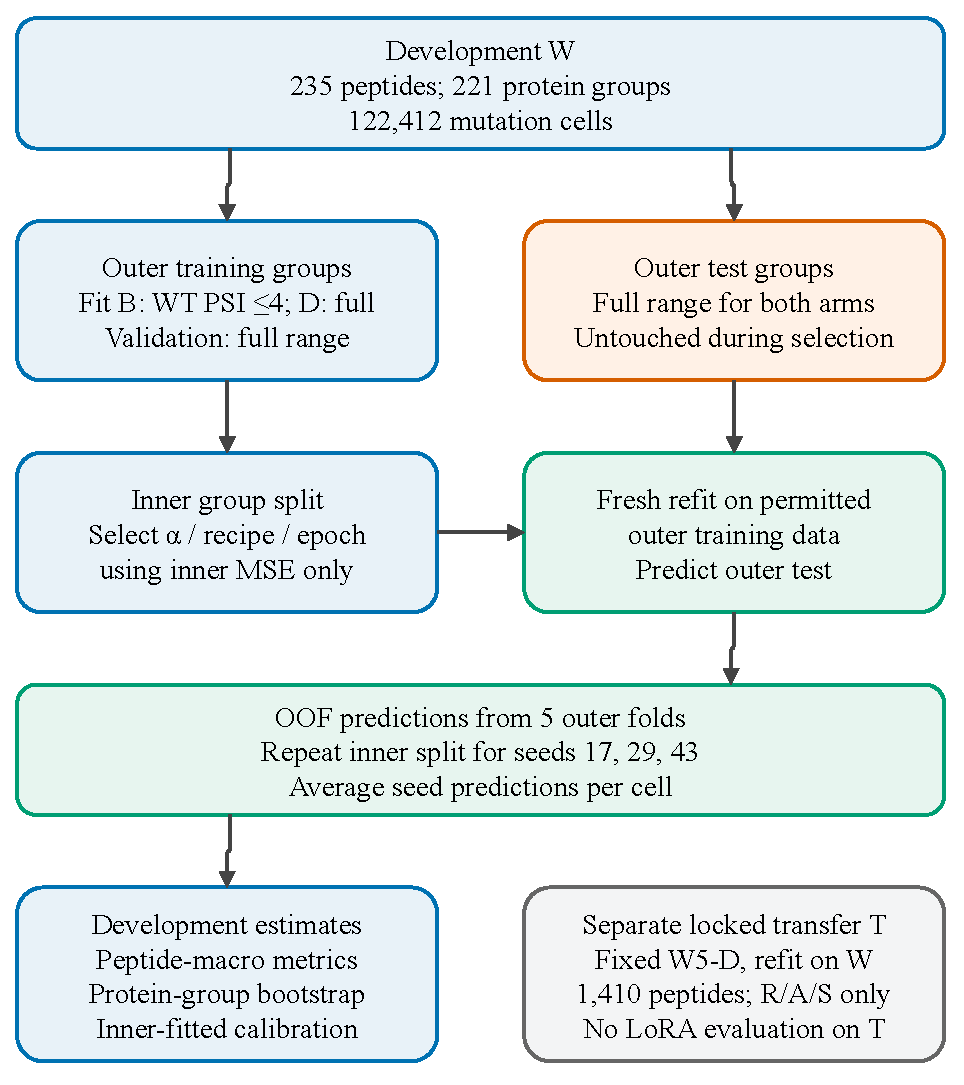
\includegraphics[width=.88\textwidth]{assets/diagrams/campaign-2026-11-06/nested-evaluation.pdf}
  \caption{Group-aware selection and evaluation. The three seed predictions are averaged per cell
  before computing ensemble metrics. The separate transfer set T evaluates the fixed W5-D recipe.}
  \label{fig:campaign-nested}
\end{figure}

\subsection{Frozen Features and Matched Adaptation}\label{sec:campaign-adaptation}
The family experiment includes ESM2 at 8M, 35M, 150M and 650M parameters, ESM1b-650M,
one ESM1v-650M checkpoint, ESM-C-300M, the ProtT5 encoder and Ankh-base. For each substitution,
the mutant-minus-WT residue embedding at the mutation site is concatenated with its sequence mean.
Frozen features are reduced to 64 principal components using training-only transforms and combined
with either the common auxiliary features alone or additional ordered W5 context. Ridge regularisation
is chosen from $\{0.1,1,10,100,1000\}$ by inner MSE. The design has
$9\times2\times2\times3\times5=540$ outer fits.

The second experiment holds ESM2-35M, the group folds, auxiliary inputs, head initialisation and
training schedule common between frozen and LoRA branches. Both use a 64-unit ReLU head with
dropout 0.2. LoRA~\citep{hu2022lora} adds rank-8 adapters with scale $16/8$ to attention query and
value projections while retaining frozen pretrained weights. The frozen branch trains the head only.
Both branches use AdamW, learning rate $10^{-4}$, weight decay 0.01, batch size 8, FP32 computation
and gradient clipping at 1. Inner selection permits at most 20 epochs with patience 4, followed by
a fresh outer refit for the selected epoch count. The backbone remains in evaluation mode in both
branches so that its dropout policy is matched. There are 30 outer fits per branch.

The local environment is Python 3.11.9, PyTorch 2.13.0 with CUDA 13.0, Transformers 5.17.0 and
an RTX 5060 Laptop GPU with approximately 8~GiB memory. Model/tokenizer weights are cached and
revision-pinned. ProtT5 initially reached a misleading tokenizer fallback requesting \texttt{tiktoken};
installing the missing Protobuf dependency restored its intended tokenizer. Ankh uses the original
fast tokenizer with residue-level input and an FP32 encoder because FP16 hidden states were
non-finite. ProtT5 uses FP16 encoding; stored family features use FP16. These execution choices are
recorded parts of the recipes, so this is not a controlled comparison of pretraining alone.

\subsection{Uncertainty, Calibration and Transfer Boundaries}
MAE is first averaged within a peptide and then across peptides. Positive-event metrics use
$\Delta\mathrm{PSI}\ge1$; negative-event metrics use $\Delta\mathrm{PSI}\le-1$ and require at least
three cells from each class within a peptide. Paired differences are bootstrapped over protein
groups with 5,000 resamples. Four matched local contrasts (two arms, MAE and positive AUROC)
are additionally reported with conservative post-hoc Bonferroni 98.75\% intervals. This adjustment
does not turn the development expansion into a preregistered independent confirmation.

Three-class probabilities represent negative, neutral and positive effects. Each outer-fold
calibrator is fitted using predictions on its inner validation groups, disjoint from the outer test;
probabilities are averaged across seeds. The multiclass Brier score is
$\sum_{c=1}^{3}(p_c-y_c)^2$ per cell, without division by the number of classes. Both cell-micro and
peptide-macro averages are reported. A null predictor uses inner-validation class frequencies;
positive-event ECE uses ten equal-width probability bins. Calibration is evaluated out of fold,
separately from final serving-model construction.

For transfer, W5-D is fixed before inspecting T, refitted on all permitted W data, and applied to
the locked scanning population with no recorded protein-group overlap with W or scanning development
data. T has a different substitution/label distribution and comes from a previously explored source
in the same laboratory. It does not provide a new independent external cohort. No LoRA model is
selected or evaluated using T in the completed campaign.
